\section{State of the Art}

\subsection{Image Sensors}

Image sensors detect and measure changes in light intensity, convening the information onto arrays of individual
points. They are found in a myriad of devices, from consumer electronics, such as cell phones, to high-end 
digital cameras, and even scientific equipment such as telescopes and microscopes. 

There are two types of digital image sensors - charged-coupled device (CCD), and active-pixel sesnsor (APS).
The following will revolve around APSs, as they are most common in consumer devices.

The main working principle behind image sensors is the photoelectric effect, in which photon energy is converted
to electrical impulses. This process is performed through photodetectors, such as photodiodes, photogates and 
pinned diodes. In APS sensors, there are three types of photodiodes: ``nwell / psub, n+ / psub and p+ / nwell``,
as well as two types of photogates: ``nMOS transistor gate to drain and pMOS transistor gate to drain``. \cite{stanford}

\begin{figure}[H]
    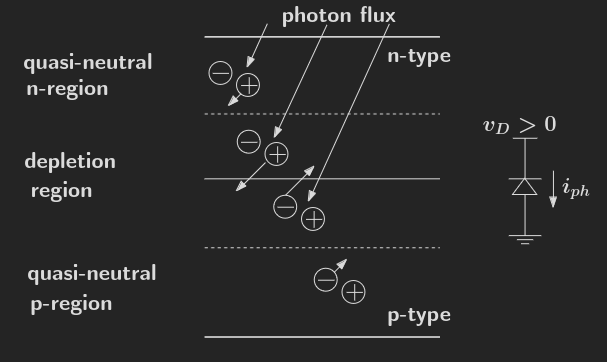
\includegraphics[width=0.35\textwidth, height=0.25\textwidth]{resources/png/photoelectric.jpg}
    \caption{Photoelectric effect. \cite{stanford} \label{figPhotoel}}
\end{figure}

Current through the diode, \(i_{ph}\) is generated by three sources of charge \cite{stanford}:
\begin{itemize}
    \item electrons in the depletion region - \(i^{sc}_{ph}\)
    \item holes generated in the quasi-neutral n-region - \(i^{p}_{ph}\)
    \item electrons generated in the quasi-neutral p-region - \(i^{n}_{ph}\)
\end{itemize}

\subsubsection{Charge gain}

The electrons generated in the depletion region are converted directly into current by a strong electric field,
while the charge carriers generated in the quasi-neutral regions need to diffuse to the depletion region in
order to be collected.

In order to obtain a measurable charge, however, the photodetector needs to be exposed to light for a period denoted
as ``integration time``, \(t_{int}\). After the integration time, the output can be measured as charge, \(Q(t_{int})\),
or as voltage, \(v_{0}(t_{int})\).

The accumulated charge can be computed with the following \cite{stanford}:

\begin{equation}
    \label{eqCharge}
    Q(t_{int}) = \frac{1}{q} (i_{ph} + i_{dc}) t_{int}
\end{equation}

where \(q\) is the electron charge, and \(i_{dc}\) is the ``dark current``, present even when no light hits the 
photodetector. Because the ``well capacity``, denoted by \(Q_{max}\), is a known manufacturing constant, the maximum
current that can be produced by each pixel can be computed as:

\begin{equation}
    \label{eqMaxCurr}
    i^{max}_{ph} = \frac{qQ_{max}}{t_{int}} - i_{dc}
\end{equation}

\begin{figure}[H]
    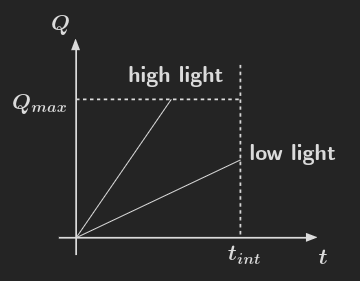
\includegraphics[width=0.35\textwidth, height=0.35\textwidth]{resources/png/integration.png}
    \caption{Charge accumulation. \cite{stanford} \label{figIntegration}}
\end{figure}

As expected, \ref{figIntegration} showcases that the gained charge is proportional to the integration time, as well
as the quantity of light hitting the sensor, with the low light measurement being capped by \(t_{int}\) and the high
luminosity measurement being capped by \(Q_{max}\).

The photodiode alone is not sufficient to accurately measure the and store the image data, thus several inputs need to
be provided alongside the light intensity in order for a pixel to function:

\begin{figure}[H]
    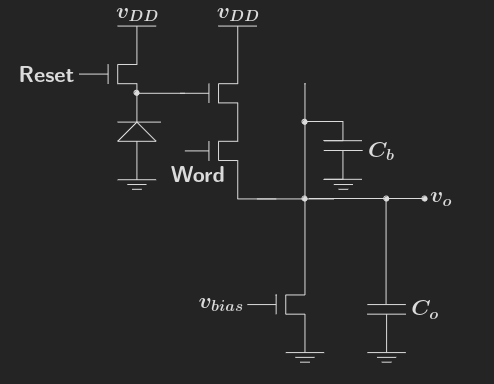
\includegraphics[width=0.35\textwidth, height=0.35\textwidth]{resources/png/pixel.png}
    \caption{APS photodiode pixel. \cite{stanford} \label{figPixel}}
\end{figure}

From \ref{figPixel}, inputs \(Reset\) and \(Word\) dictate when a pixel value should be set to \(i_{dc}\), respectively
when its value should be read. Output \(v_{0}\) is written to the storage capacitor \(C_{0}\) whenever the values
is requested, and from there it is passed along for further processing.

Individual pixels can only measure the incident light in a small surface area, thus they are grouped into arrays, with 
common inputs for each row, and common outputs for each column:

\begin{figure}[H]
    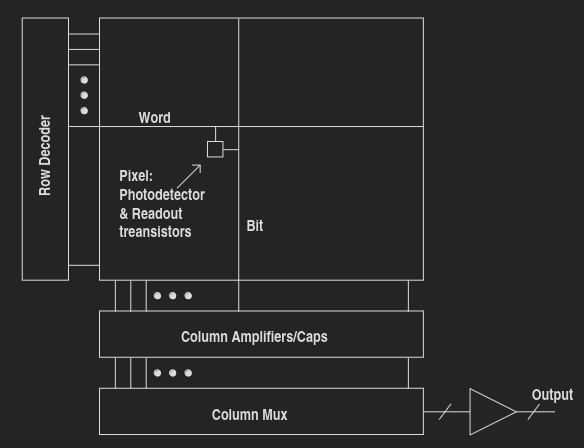
\includegraphics[width=0.45\textwidth, height=0.45\textwidth]{resources/png/lattice.png}
    \caption{Image sensor pixel lattice. \cite{stanford} \label{figLatice}}
\end{figure}

For most APS sensors, in the diagram from \ref{figLatice}, the row decoder sequential activates each pixel row for recording
and output, with the values being sent in parallel to the column capacitors. Due to this behavior, called a ``rolling shutter``, 
the environment might change between two consecutive row readouts.

\subsubsection{Noise}

Due to the dark current, \(i_{dc}\), spots of increased luminosity can be falsely read onto the final image, resulting in noise
patterns. Most prevalent in APS sensors is fixed pattern noise (FPN), denoted as such because it is fixed for each sensor.
For APSs specifically, FPN is most noticeable across columns, due to amplification, leading to stripes in the final image. \cite{stanford}

Additionally, fixed pattern noise can be caused by variations in pixel parameters and is quantified as ``standard 
deviation of the spatial variation in pixel outputs under uniform illumination``, with reported experimental
deviations of \(<1\%\) to \(>4\%\).

\subsection{Dynamic Range}

Dynamic Range (DR) represents the ratio between the highest and lowest recorded pixel values. 
Measured in \(dB\), it can be represented by 

\begin{equation}
    \label{eqDR}
    DR = 20log_{10}(\frac{i_{max}}{i_{min}})
\end{equation}

where \(i_{max}\) and \(i_{min}\) represent the maximum, and minimum intensities. 

\begin{figure}[H]
    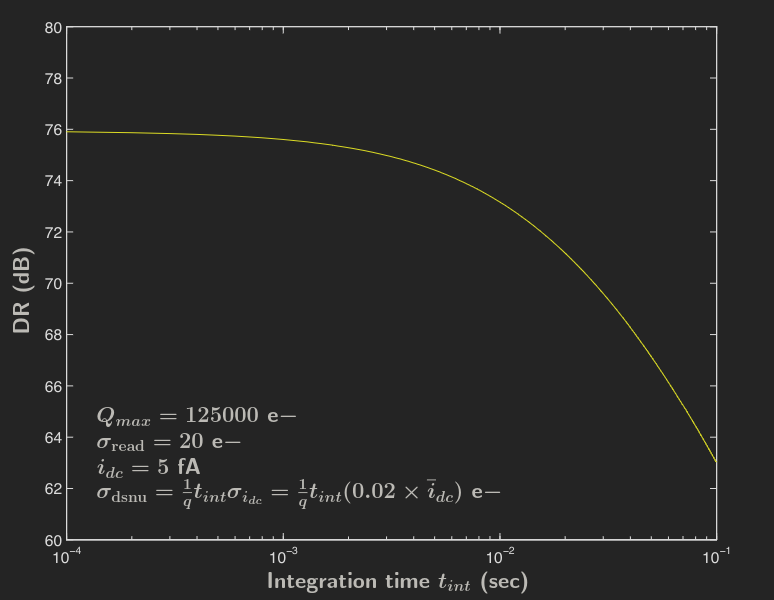
\includegraphics[width=0.55\textwidth, height=0.50\textwidth]{resources/png/drgraph.png}
    \caption{Dynamic range versus integration time. \cite{stanford} \label{figDR}}
\end{figure}

With the value of each pixel increasing linearly with the integration time \(t_{int}\), it follows that the \(DR\) will decrease as all pixels 
approach saturation, as seen in \ref{figDR}. \cite{stanford}

Due to the aforementioned limitation, the dynamic range of most consumer grade sensors is severely limited, 
when compared to the scenes meant for capture.

Dynamic range varies for different capture devices with the human eye averaging around \(90dB\), 
CCDs between \(66dB\) and \(>78dB\), and consumer APSs at around \(54dB\). \cite{stanford}

As a consequence, there is a constant research towards increasing the dynamic range of CMOS sensors, with a constant
balance between increasing the maximum intensity, decreasing the dark current and managing timing and storage
constraints. Each of those parameters can be a source of noise, another facet that needs to be accounted
for when researching image sensor improvements.

\subsection{Methods of Increasing Dynamic Range}

\subsubsection{Multi-Sampling}

Multi-sampling refers to the sequential capture of two identical frames, with different integration times, in order
to capture both high and low light regions. In the particular case of dual sampling, the same row is read twice,
with a reset between each read. The resulting images are passed along to a designated processing unit, where
they can be combined linearly (through bit concatenation) or non-linearly (through addition). \cite{withSampling}

Another technique researched is that of ``Predictive Multiple Sampling``, in which a selected interval is
used as a reference point for a set of shorter integration times, all having a common end point. Out of this set,
an optimal interval is chosen based on recorded pixel values ``while a pixel saturation predictive decision 
is used to overlap the integration intervals within the given integration time such that only one frame 
using the optimal integration interval for each pixel is produced``. \cite{withPredictive}

Experimental results for both methods showcase a possible dynamic range of \(70-108dB\), at the expense of
increased noise distortion. \cite{withSampling, withPredictive}

\subsubsection{Time to Saturation}

This method relies on different integration times for each pixel, requiring the addition of signal processing
components directly into the sensor circuitry. The process can vary, depending on weather the image is to
be used by itself or in a video stream.

For single images, the intensity \(i_{ph}\) can be computed as

\begin{equation}
    \label{eqIph}
    i_{ph} = 
    \begin{cases}
        \frac{qQ_{max}}{t_{sat}}, \text{ } i_{ph} > \frac{qQ_{max}}{t_{int}} \\
        i_{ph}, \text{ } i_{ph} < \frac{qQ_{max}}{t_{int}} \\
    \end{cases}
\end{equation}

where \(t_{sat}\) is the saturation time of the photodetector. In this case, the additions to the circuit conssit
of a comparator, and a capacitor used to store the duration. Both the input from the diode, as well as the 
time-stamp, are passed to an ADC, with the computation being done in the digital domain. \cite{stanford}

Another implementation is based on a sequence of frames, with the previous readout influencing the one currently
occurring. In this case, after every integration interval, a check for saturation or ``motion`` is performed on
each pixel. This is done through a comparison between the current pixel charge and the previous report, based
on a given threshold value \(th_{m}\). If the difference between the two values exceeds the threshold, both values
are sent to the controlling circuit. At the same time, saturation is also checked for, using a different 
threshold, \(th_{s}\), in which case the voltages are again sent to the main circuit, and the photodetector is
reset. If neither condition is met, no output is provided, and the diode continues to integrate. \cite{withTime}

This method is able to achieve a dynamic range of 56dB, but it is costly both in terms of circuit complexity, as 
well as power consumption. \cite{stanford, withTime}

\subsubsection{Linear-Logarithmic Response}

The approach used in this project, this method relies on changing between a linear response to the charge on
the photodiode, to a logarithmic one, based on a given threshold value. Due to the different characteristic
curves, an increased dynamic range is achieved by having an increased range of resulting values, when compared
to each individual response.

\begin{figure}[H]
    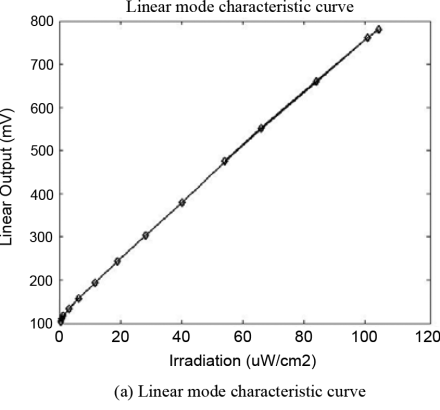
\includegraphics[width=0.49\textwidth, height=0.50\textwidth]{resources/png/linGraph.png}
    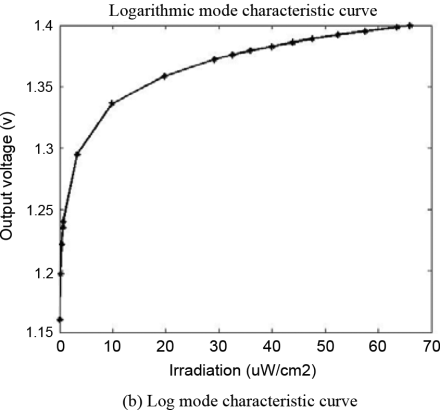
\includegraphics[width=0.49\textwidth, height=0.50\textwidth]{resources/png/logGraph.png}
    \caption{Linear and logarithmic characteristic curves. \cite{withScience} \label{figCurves}}
\end{figure}

As showcased in \ref{figCurves}, for low light conditions the linear response provides a greater range of values
for low light intensity, with the output voltage spiking as luminosity increases. In contrast, the logarithmic
response provides little accuracy for low light, with the output values clumping as the intensity spikes.

\begin{figure}[H]
    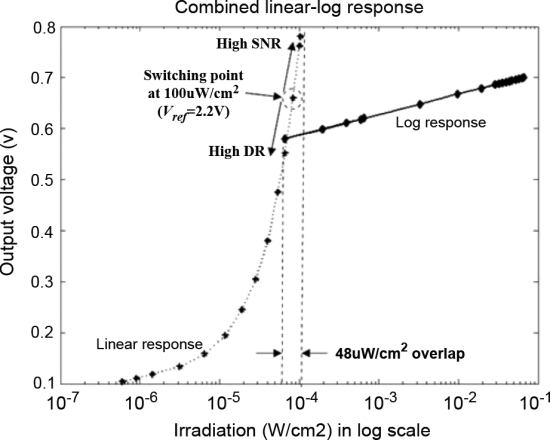
\includegraphics[width=0.55\textwidth, height=0.50\textwidth]{resources/png/combinedGraph.png}
    \caption{Combined characteristic curve. \cite{withScience} \label{figCurveCombined}}
\end{figure}

Because of the exponential nature of the charge gain, combining the two responses generates a better coverage
of the entire luminosity spectrum, as shown in \ref{figCurveCombined}.

